\section{Methodology of \tool}

\begin{figure*}[ht]
    \centering
      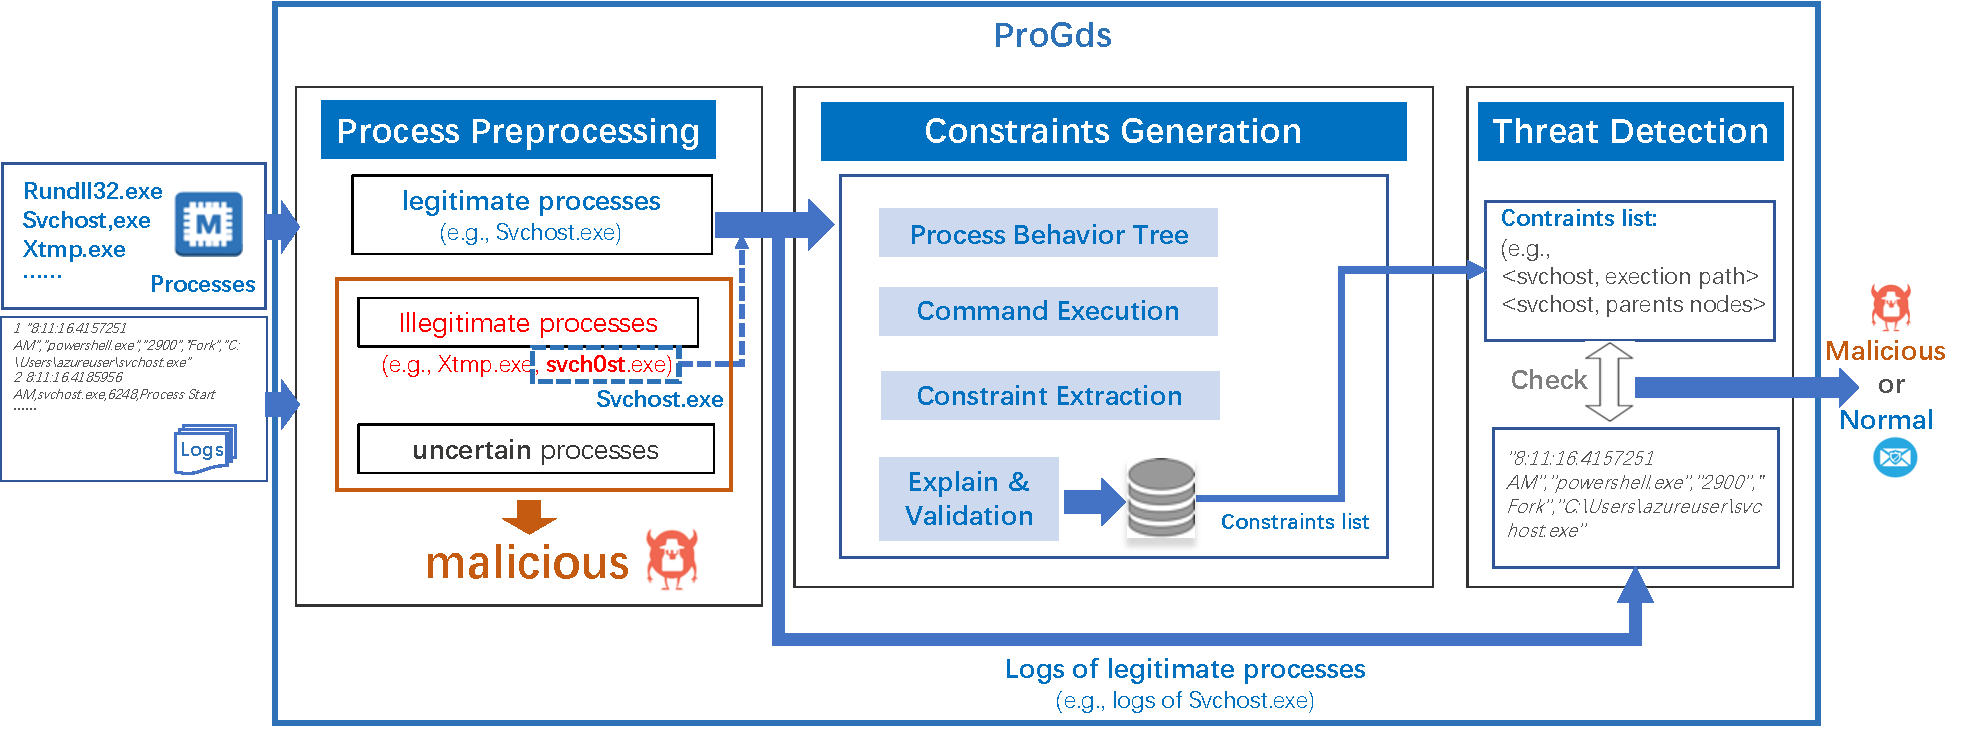
\includegraphics[width=0.95\textwidth]{figs/overview.pdf}
      % \caption{An overview of \tool.}
    \caption{The system process logs are collected and categorized using LLM as legitimate, illegitimate, and uncertain processes. Processes labeled uncertain or illegitimate are flagged for security analyst review (detailed in Section~\ref{sec:classifition}). If determined to be legitimate, LLM assists in the creation of a database of process constraints. This is achieved through behavior tree creation, command execution, constraint extraction and validation (explained in Section~\ref{sec:profile_con}). Logs that violate these constraints are indicative of potential threats (detailed in Section~\ref{sec:Threat_detection}).}
    \label{fig-framework}
    \end{figure*}

\subsection{Threat Model}\label{sec:threatModel}
In this paper, we consider APT attacks targeting critical entities that have been identified as critical infrastructure, and these attacks have the following characteristics:

\begin{itemize}
    \item \textbf{Stealthy}. The attacker employs covert tactics, concealing their malicious activities amid a substantial volume of benign background data, resulting in the victim system exhibiting behavior akin to a benign mode.
    \item \textbf{Evolving}. Professional attacker groups continually innovate, extending their targets to a broader array of system processes and adeptly adjusting to the latest defensive mechanisms to maintain a competitive edge.
    %As professional attacker groups continue to innovate, they are targeting an ever-expanding range of system processes and adapting to the latest defensive measures in order to stay ahead of the game. 
    \item \textbf{Frequent usage of zero-day exploits}. The attacker primarily relies on zero-day exploits, resulting in a lack of advance knowledge w.r.t. the specific attack patterns.
\end{itemize}
% Note that, as an alternative to sample-focused analysis, we propose to observe ubiquitous OS kernel processes. The system processes are always present and do not need to be identified before analysis, unlike suspicious samples.

\subsection{Technical Challenges}\label{sec:challenges}
A straightforward idea is to utilize the knowledge extraction capabilities in LLMs to facilitate the construction of more comprehensive profiles and constraints for victim system processes first, which can then be employed for conducting further thorough attack detection analysis. Recall that,
when dealing with the evolution of attacks or their stealthy tactics, supplemental knowledge can be very crucial. Moreover, in contrast to learning-based detection methods, this approach obviates the requirement for pre-defined attack patterns, which also enhances its adaptability and versatility in addressing evolving threat landscapes.
%How can we efficiently extract these constraints? It's a crucial question. Fortunately, LLMs offers significant advantages when it comes to building process profiles due to its exceptional knowledge extraction capabilities.
However, the direct employment of LLMs in our setting gives rise to the following three notable technical challenges:

% \circled{1} Complexity Handling: It might be difficult for LLMs to give comprehensive solutions when they are faced with complicated questions or scenarios.

\noindent
{\bf CH-\circled{1} Context Dependency.} %  : 
To achieve precise outcomes, LLMs commonly necessitate an enriched contextual environment. In the absence thereof, their responses may exhibit a propensity towards generality or imprecision. However, ... \yd{YD: Add statement about "hardness in our setting to get enriched context environment directly"}

\noindent
{\bf CH-\circled{2} Memory Limitations.} % \circled{2}
\yd{YD: Add statement about facts w.r.t long context in our setting.} However, owing to the constraints imposed by their token limits, LLMs encounter challenges when confronted with exceedingly lengthy texts. Moreover, LLMs exhibit a proclivity for prioritizing recent interactions, often at the expense of overlooking pertinent details embedded within the broader context of prior conversational history.
% Due to its token limit, LLMs cannot handle excessively long texts. In addition, LLMs tend to focus more on recent interactions and overlook previous details in a conversation history. 

\noindent
{\bf CH-\circled{3} Hallucination Problems.} % \circled{3} 
In spite of the remarkable advancement of LLMs in excelling across a diverse spectrum of understanding tasks, these intelligent models still show a significant drawback: the tendency to `hallucinate', i.e., they may generate misinformation and lead to unsafe behaviors.\yd{YD: Add refers about Hallucination.}
% This risk entails
In this work, such a risk entails the possibility of the model generating information for a given system process that appears plausible at first glance but lacks factual support or corresponds to non-existent realities.
% that might reveal plausible-looking yet factually unsupported or nonexistent information if the model does produce hallucinations. 

% Therefore, the key to building process profiles using LLMs is overcoming these challenges which is the central focus of this paper.

\subsection{Overview of \tool}
In this work, we propose an effective LLMs-based APT attack detection framework, named \tool, addressing all the above challenges. The overview of \tool can be found in Figure~\ref{fig-framework}. 

\tool comprises three main components: Process Preprocessing, Constraints Generation, and Threat Detection.
Given a bundle of logs collected from a variety of system processes, \tool first conducts an LLMs-based process preprocessing procedure to filter out processes with legitimate names and transmit these names into the Constraints Generation component, while concurrently forwarding the detailed logs of the legitimate processes to the Threat Detection component. Note that, in cases where illegitimate processes share names resembling those of legitimate counterparts, \tool not only identifies and corrects them but also categorizes them as legitimate processes. For other illegitimate or uncertain processes, \tool classifies them as potentially malicious ones. Then, the LLMs-based Constraints Generation component constructs a database for all the legitimate processes received from the previous step, outlining the typical constraints associated with the processes. Finally, the Threat Detection component checks the consistency between the constraints generated and the original logs, and any violation of these constraints will be indicated as a malicious activity.

To address the technical challenges outlined in Section~\ref{sec:challenges}, we decompose the Constraints Generation component into four LLMs-manageable subtasks.


% As illustrated in Figure~\ref{fig-framework}, we accessed a log collection tool to collect logs from a variety of system processes that were running at different times in the system. Utilizing the powerful capabilities of LLMs, we were able to categorize these processes based on their names into three distinct categories: legitimate process names, illegitimate process names, and uncertain process names (due to the inherent incompleteness of the GPT's database). As for the latter two categories, we classified them as potentially malicious, requiring more investigation by security analysts in order to determine whether they are malicious or not. A more in-depth examination of this process is provided in Section~\ref{sec:classifition}.

% As for processes that were classified with legitimate names, we used the LLMs to construct a database that outlined the normal constraints of the process.

% In a previous Section~\ref{sec:intuition}, we briefly discussed the four challenges that exist when building process profiles based on the LLMs model. To address these challenges, we developed ProfileGuard, a method that harnesses LLMs for the automated creation of critical system process profiles based on the information provided by LLMs. ProfileGuard acts as a security guard for the system, using system process profiles to prevent malicious attackers.
% We broke down the comprehensive profiling task into four manageable subtasks:
\noindent
{\bf Process Behavior Tree Construction.} To provide an enriched contextual environment for LLMs, we first capture a comprehensive range of behaviors for each process, i.e., creating a behavior tree for each process. Then, the Large Language Model (LLM) continuously expands its knowledge of this behavior tree through a ``self-ask" manner. Finally, the LLM benefits greatly from this behavior tree as it provides an enriched contextual environment, which can greatly tackle the challenge {\bf CH-\circled{1}}.

\noindent
{\bf Command Execution.} The behavior tree can then be used to guide the LLMs to script and execute commands for behaviors that could be addressed. In addition, command execution generates richer contextual information for {\bf CH-\circled{1}}, and checks simple constraints, such as execution paths and parent-child relationships. \yd{YD: Recheck and Refine.}

\noindent
{\bf Constraint Extraction.} In this step, we'll combine the LLMs and traditional programs to solve {\bf CH-\circled{2}}. Since the log size is large, asking GPT directly will easily exceed its memory limit and cause previous information to be lost. We employed common term and prefix-span sequence mining to discover deeper relationships between logs. Each constraint, which was identified by LLMs, was interpreted using its knowledge. \yd{YD: Recheck and Refine.}

\noindent
{\bf Explanation \& Validation.} LLMs must be accurate and consistent due to potential hallucination issues. We've implemented a two-tier validation approach to validate the model's outputs for {\bf CH-\circled{3}}. The first tier involves executing actual commands and cross-checking with real-world logs. Multiple LLMs engage in a multi-round debate to mutually verify their respective responses and reasoning, aiming to arrive at a unified conclusion. \yd{YD: Recheck and Refine.}
% \begin{itemize}
%     % \item \textbf{Process Behavior Tree Construction}: Our goal was to capture a comprehensive range of behaviors for each process, creating a behavior tree. Through a "self-ask" approach, the LLMs continuously expanded its knowledge of this tree. LLMs can benefit greatly from this tree as it provides context for {\bf CH-\circled{1}}.
%     % \item \textbf{Command Execution}: A behavior tree was used to guide the LLMs to script and execute commands for behaviors that could be addressed. In addition, command execution generates richer contextual information for {\bf CH-\circled{1}}, and checks simple constraints, such as execution paths and parent-child relationships.
%     % \item \textbf{Constraint Extraction}:  In this step, we'll combine the LLMs and traditional programs to solve {\bf CH-\circled{2}}. Since the log size is large, asking GPT directly will easily exceed its memory limit and cause previous information to be lost. We employed common term and prefix-span sequence mining to discover deeper relationships between logs. Each constraint, which was identified by LLMs, was interpreted using its knowledge.
%     \item \textbf{Validation}: LLMs must be accurate and consistent due to potential hallucination issues. We've implemented a two-tier validation approach to validate the model's outputs for {\bf CH-\circled{3}}. The first tier involves executing actual commands and cross-checking with real-world logs. Multiple LLMs engage in a multi-round debate to mutually verify their respective responses and reasoning, aiming to arrive at a unified conclusion.
% \end{itemize}

% Leveraging this process behavior database, we compared extracted log information against the established constraints. Any violation of these constraints is indicative of potential malicious activity.
% A detailed discussion on this topic is set out in Section~\ref{sec:Threat_detection}. 






